\section{Results}
The final participant-level model obtains ROC-AUC 0.8947, PR-AUC 0.8641, balanced accuracy 0.8421, macro F1 0.8421, Brier score 0.1159, calibration intercept -0.5321, and calibration slope 0.8693 with 57 predictions and zero
skipped folds (Table~\ref{tab:final-model-metrics}, Figure~\ref{fig:final-roc},
Figure~\ref{fig:final-pr}). The DFM exposure-only model is weak, while sensitivity
and residual gaze models are strong (Table~\ref{tab:dfm-exposure-sensitivity},
Figure~\ref{fig:dfm-exposure-sensitivity}). This supports the interpretation that
the signal reflects participant-level predictability sensitivity rather than the text
assigned to a participant.

The permutation test uses 1,000 valid permutations and gives $p=0.000999$.
Bootstrap intervals are [0.7765, 0.9841] for ROC-AUC and [0.7083, 0.9728] for PR-AUC
(Table~\ref{tab:robustness}, Figure~\ref{fig:permutation-null},
Figure~\ref{fig:bootstrap-auc}). Calibration and influence summaries are reported in
Table~\ref{tab:calibration-influence}, Figure~\ref{fig:calibration}, and
Figure~\ref{fig:participant-error}. Feature stability is shown in
Table~\ref{tab:feature-stability} and Figure~\ref{fig:feature-stability}.


\begin{table}[t]
\centering
\small
\caption{Locked final participant-level model metrics.}
\label{tab:final-model-metrics}
\begin{tabular}{llllll}
\toprule
analysis & split\_name & feature\_group & model & n\_features & n\_predictions \\
\midrule
phase4\_confirmatory\_participant\_prediction & leave\_one\_participant\_out & D3\_dfm\_residual\_gaze\_only & logistic\_regression & 12 & 57 \\
\bottomrule
\end{tabular}
\end{table}


\begin{table}[t]
\centering
\scriptsize
\caption{DFM exposure-only and sensitivity/residual gaze comparisons.}
\label{tab:dfm-exposure-sensitivity}
\resizebox{\linewidth}{!}{%
\begin{tabular}{lllllll}
\toprule
feature\_group & n\_features & n\_predictions & roc\_auc & pr\_auc & balanced\_accuracy & brier\_score \\
\midrule
D1\_dfm\_exposure\_only & 3 & 57 & 0.4238 & 0.3685 & 0.4474 & 0.2684 \\
D2\_dfm\_sensitivity\_only & 16 & 57 & 0.8892 & 0.8611 & 0.8421 & 0.1130 \\
D3\_dfm\_residual\_gaze\_only & 12 & 57 & 0.8947 & 0.8641 & 0.8421 & 0.1159 \\
D4\_dfm\_exposure\_plus\_sensitivity & 19 & 57 & 0.8726 & 0.8561 & 0.8158 & 0.1206 \\
\bottomrule
\end{tabular}%
}
\end{table}


\begin{table}[t]
\centering
\small
\caption{Permutation, bootstrap, and influence robustness summary.}
\label{tab:robustness}
\begin{tabular}{llll}
\toprule
test & value & n & note \\
\midrule
permutation & 0.000999000999000999 & 1000 & +1 corrected p-value \\
bootstrap\_roc\_auc & [0.7765, 0.9841] & 2000 & participant bootstrap CI \\
bootstrap\_pr\_auc & [0.7083, 0.9728] & 2000 & participant bootstrap CI \\
\bottomrule
\end{tabular}
\end{table}


\begin{table}[t]
\centering
\small
\caption{Calibration and participant influence summary.}
\label{tab:calibration-influence}
\begin{tabular}{llllll}
\toprule
brier\_score & calibration\_intercept & calibration\_slope & misclassified\_participants & high\_leverage\_participants & calibration\_bins \\
\midrule
0.1159 & -0.5321 & 0.8693 & 8.0000 & 6.0000 & 5.0000 \\
\bottomrule
\end{tabular}
\end{table}


\begin{figure}[t]
\centering
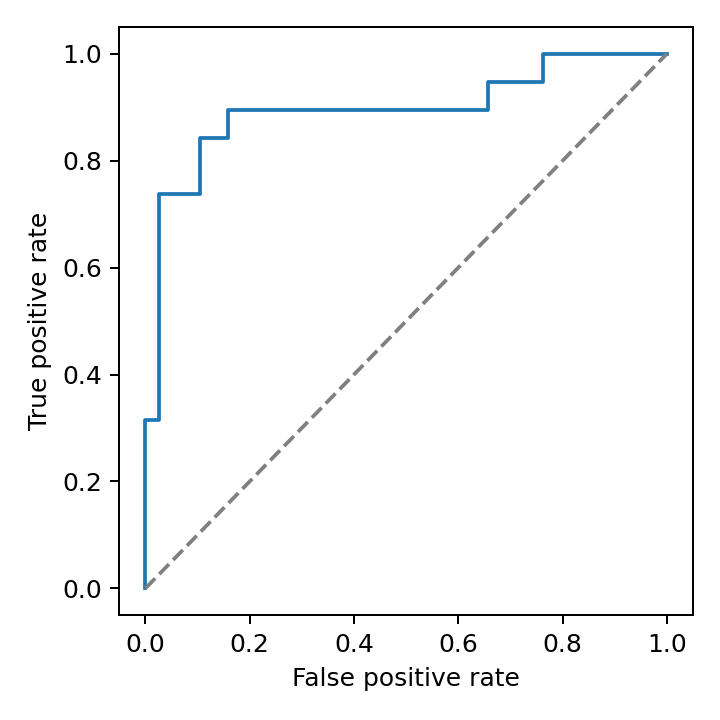
\includegraphics[width=0.92\linewidth]{figures/final_roc.png}
\caption{Final participant-level ROC curve.}
\label{fig:final-roc}
\end{figure}

\begin{figure}[t]
\centering
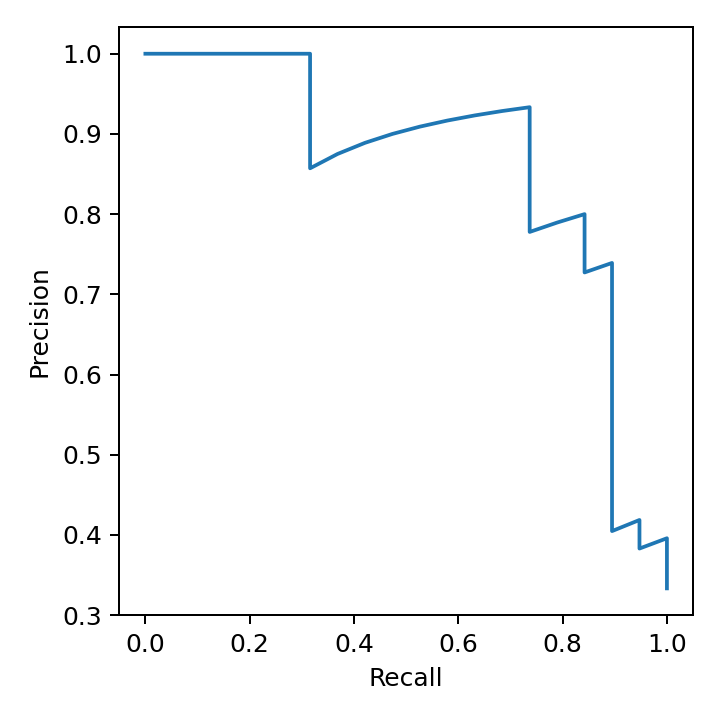
\includegraphics[width=0.92\linewidth]{figures/final_pr.png}
\caption{Final participant-level precision-recall curve.}
\label{fig:final-pr}
\end{figure}

\begin{figure}[t]
\centering
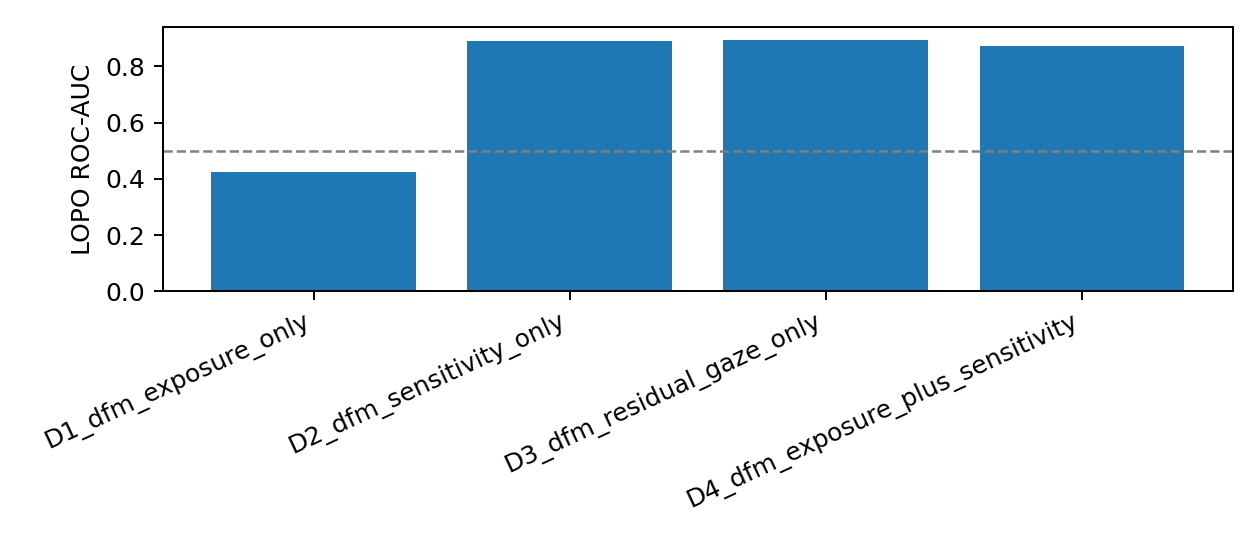
\includegraphics[width=0.92\linewidth]{figures/dfm_exposure_vs_sensitivity.png}
\caption{DFM exposure-only versus DFM sensitivity and residual gaze models.}
\label{fig:dfm-exposure-sensitivity}
\end{figure}

\begin{figure}[t]
\centering
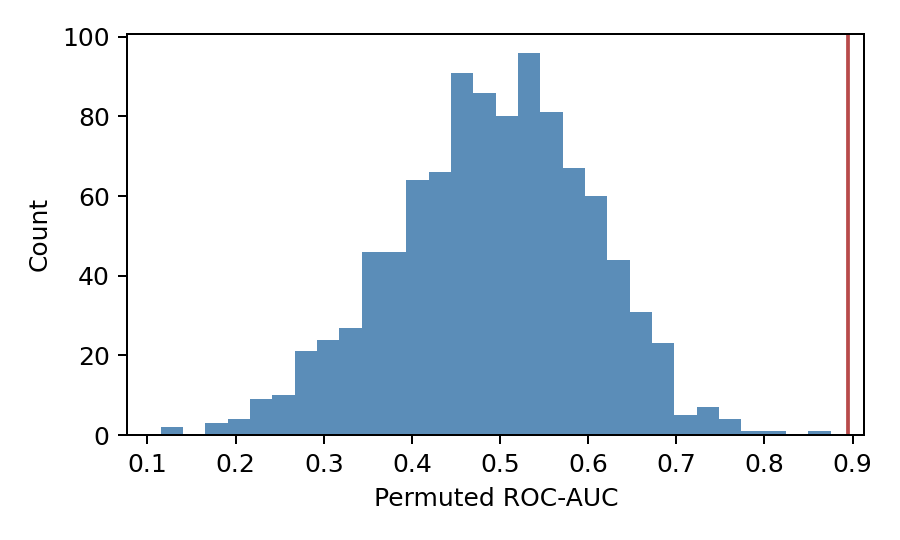
\includegraphics[width=0.92\linewidth]{figures/permutation_null.png}
\caption{Permutation null distribution for the locked final model.}
\label{fig:permutation-null}
\end{figure}

\begin{figure}[t]
\centering
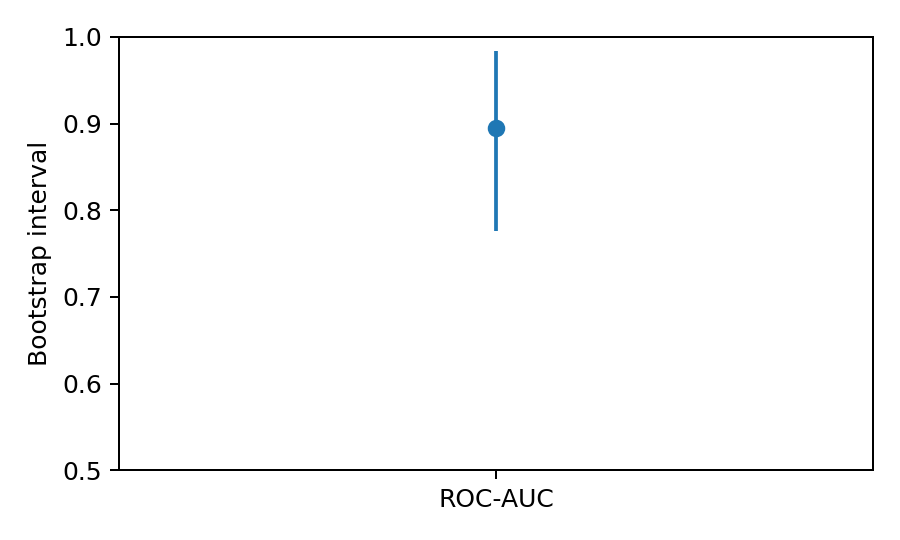
\includegraphics[width=0.92\linewidth]{figures/bootstrap_auc.png}
\caption{Bootstrap uncertainty for the final model AUC estimates.}
\label{fig:bootstrap-auc}
\end{figure}

\begin{figure}[t]
\centering
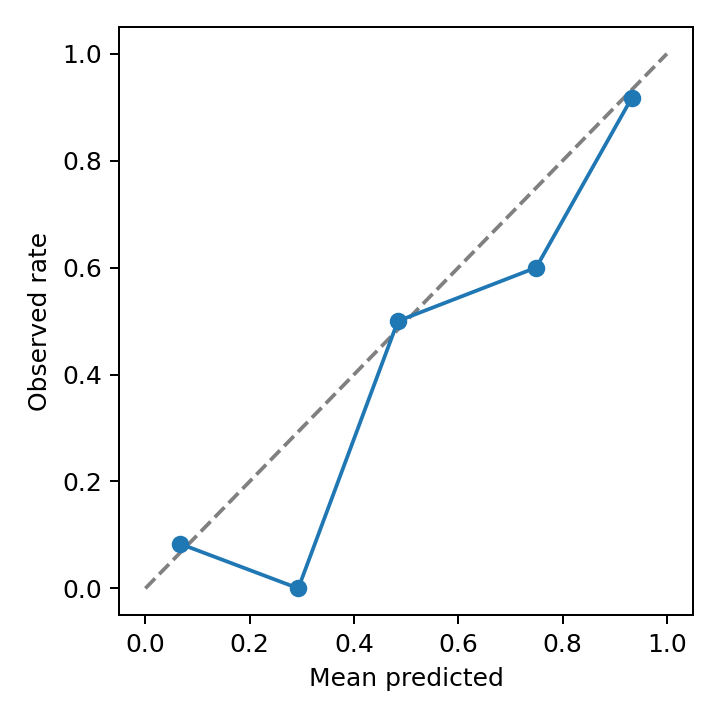
\includegraphics[width=0.92\linewidth]{figures/calibration.png}
\caption{Calibration summary for the final participant-level predictions.}
\label{fig:calibration}
\end{figure}

\begin{figure}[t]
\centering
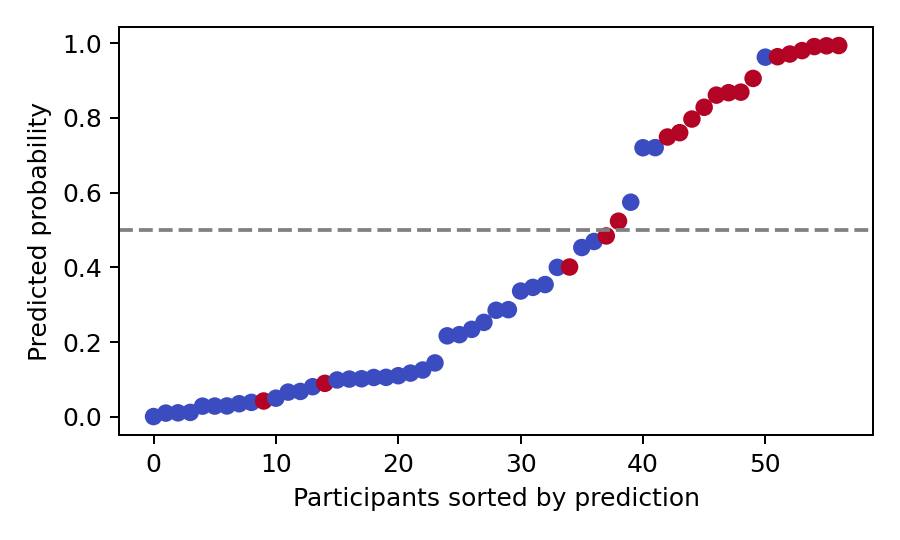
\includegraphics[width=0.92\linewidth]{figures/participant_error.png}
\caption{Participant-level prediction error and influence audit.}
\label{fig:participant-error}
\end{figure}

\begin{figure}[t]
\centering
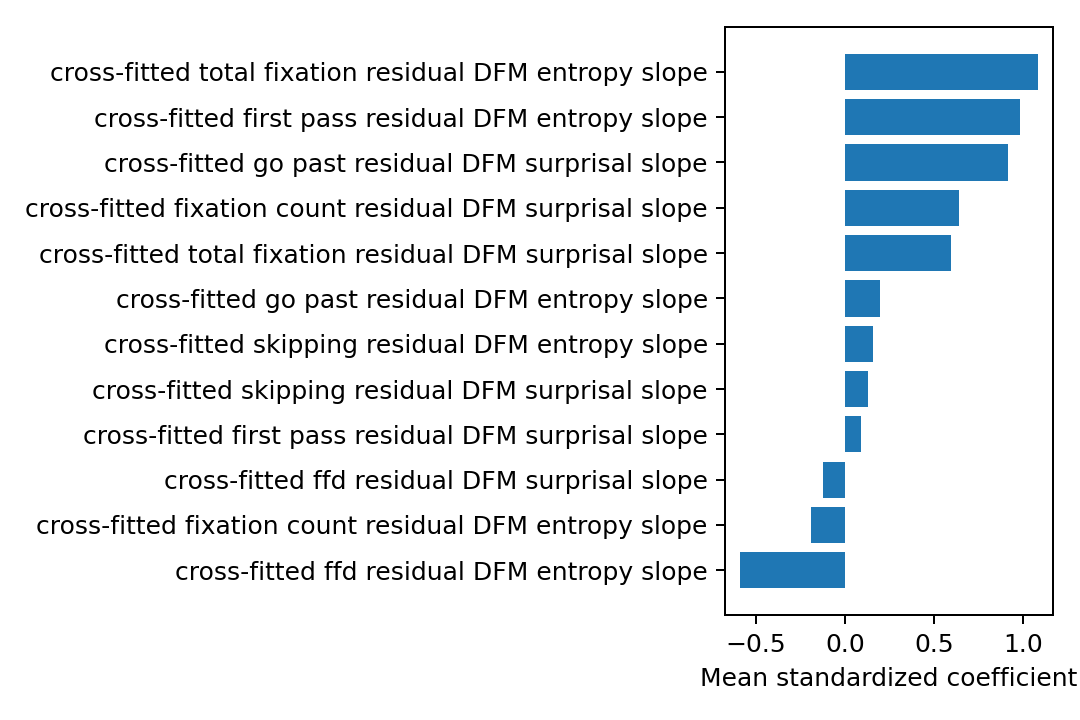
\includegraphics[width=0.92\linewidth]{figures/feature_stability.png}
\caption{Coefficient stability for DFM residual gaze features.}
\label{fig:feature-stability}
\end{figure}
